\section{External Memory Module}
\begin{figure}[h!]
    \centering
    \vspace{1em}
\scalebox{0.85}{
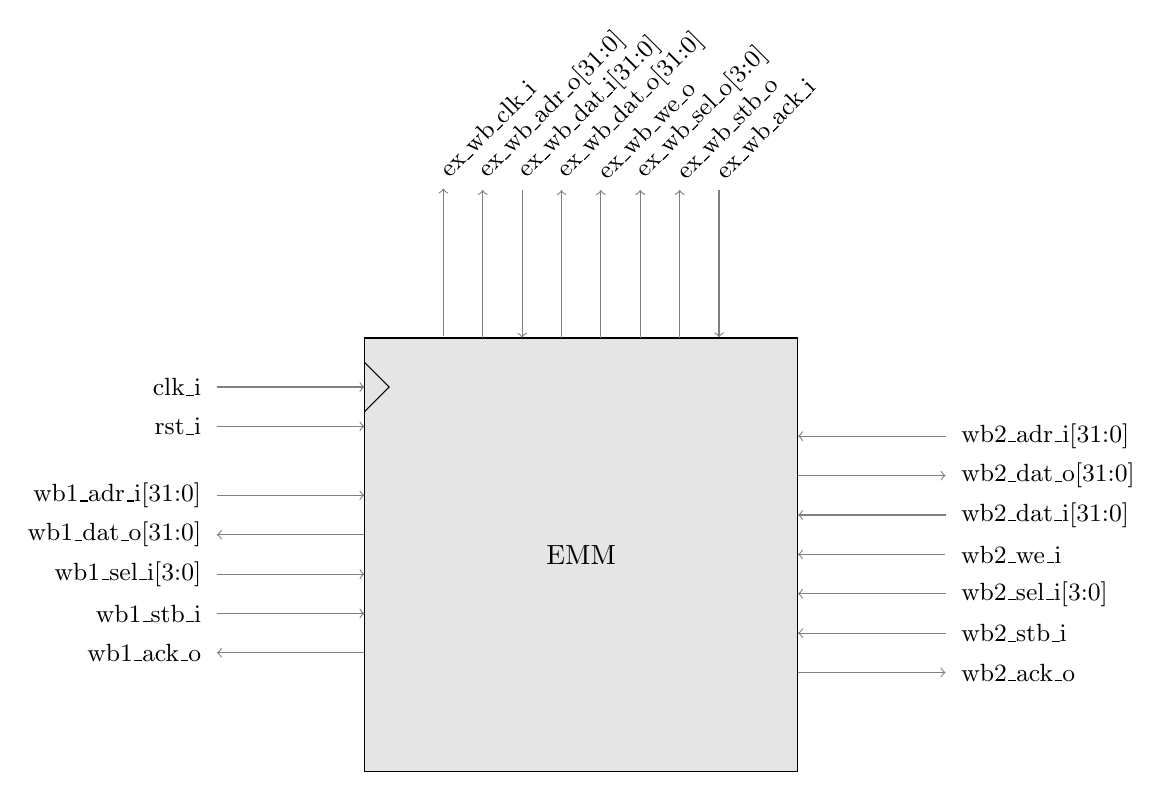
\begin{tikzpicture}[scale=1.25, draw=gray, inner sep=0, outer sep=0]
  \node[rectangle, draw=black,
    anchor=south,
    align=center,
    minimum height = 5.5cm,
    minimum width = 5.5cm,
    fill = gray!20] (block) at (0, 0) {EMM};

  \node (rport4) at (block.east) {};
  \node (rport3) at ([yshift=0.4cm]rport4.center) {};
  \node (rport2) at ([yshift=0.4cm]rport3.center) {};
  \node (rport1) at ([yshift=0.4cm]rport2.center) {};
  \node (rport5) at ([yshift=-0.4cm]rport4.center) {};
  \node (rport6) at ([yshift=-0.4cm]rport5.center) {};
  \node (rport7) at ([yshift=-0.4cm]rport6.center) {};
  \draw[->] ([xshift=1.5cm]rport1.center) node[right=0.2cm, anchor=west]{\small wb2\_adr\_i[31:0]} -- (rport1.center);
  \draw[<-] ([xshift=1.5cm]rport2.center) node[right=0.2cm, anchor=west]{\small wb2\_dat\_o[31:0]} -- (rport2.center);
  \draw[->] ([xshift=1.5cm]rport3.center) node[right=0.2cm, anchor=west]{\small wb2\_dat\_i[31:0]} -- (rport3.center);
  \draw[->] ([xshift=1.5cm]rport4.center) node[right=0.2cm, anchor=west]{\small wb2\_we\_i} -- (rport4.center);
  \draw[->] ([xshift=1.5cm]rport5.center) node[right=0.2cm, anchor=west]{\small wb2\_sel\_i[3:0]} -- (rport5.center);
  \draw[->] ([xshift=1.5cm]rport6.center) node[right=0.2cm, anchor=west]{\small wb2\_stb\_i} -- (rport6.center);
  \draw[<-] ([xshift=1.5cm]rport7.center) node[right=0.2cm, anchor=west]{\small wb2\_ack\_o} -- (rport7.center);

  \node(uport4) at ([xshift=-0.2cm]block.north) {};
  \node(uport3) at ([xshift=-0.4cm]uport4.center) {};
  \node(uport2) at ([xshift=-0.4cm]uport3.center) {};
  \node(uport1) at ([xshift=-0.4cm]uport2.north) {};
  \node(uport5) at ([xshift=0.4cm]uport4.center) {};
  \node(uport6) at ([xshift=0.4cm]uport5.center) {};
  \node(uport7) at ([xshift=0.4cm]uport6.center) {};
  \node(uport8) at ([xshift=0.4cm]uport7.center) {};
  \draw[<-] ([yshift=1.5cm]uport1.center) node[above=0.2cm, anchor=west, rotate=45]{\small ex\_wb\_clk\_i} -- (uport1.center);
  \draw[<-] ([yshift=1.5cm]uport2.center) node[above=0.2cm, anchor=west, rotate=45]{\small ex\_wb\_adr\_o[31:0]} -- (uport2.center);
  \draw[->] ([yshift=1.5cm]uport3.center) node[above=0.2cm, anchor=west, rotate=45]{\small ex\_wb\_dat\_i[31:0]} -- (uport3.center);
  \draw[<-] ([yshift=1.5cm]uport4.center) node[above=0.2cm, anchor=west, rotate=45]{\small ex\_wb\_dat\_o[31:0]} -- (uport4.center);
  \draw[<-] ([yshift=1.5cm]uport5.center) node[above=0.2cm, anchor=west, rotate=45]{\small ex\_wb\_we\_o} -- (uport5.center);
  \draw[<-] ([yshift=1.5cm]uport6.center) node[above=0.2cm, anchor=west, rotate=45]{\small ex\_wb\_sel\_o[3:0]} -- (uport6.center);
  \draw[<-] ([yshift=1.5cm]uport7.center) node[above=0.2cm, anchor=west, rotate=45]{\small ex\_wb\_stb\_o} -- (uport7.center);
  \draw[->] ([yshift=1.5cm]uport8.center) node[above=0.2cm, anchor=west, rotate=45]{\small ex\_wb\_ack\_i} -- (uport8.center);

  \node (lport3) at ([yshift=-0.2cm]block.west) {};
  \node (lport2) at ([yshift=0.4cm]lport3.center) {};
  \node (lport1) at ([yshift=0.4cm]lport2.center) {};
  \node (lport4) at ([yshift=-0.4cm]lport3.center) {};
  \node (lport5) at ([yshift=-0.4cm]lport4.center) {};

  \draw[->] ([xshift=-1.5cm]lport1.center) node[left=0.2cm, anchor=east]{\small wb1\_adr\_i[31:0]} -- (lport1.center);
  \draw[<-] ([xshift=-1.5cm]lport2.center) node[left=0.2cm, anchor=east]{\small wb1\_dat\_o[31:0]} -- (lport2.center);
  \draw[->] ([xshift=-1.5cm]lport3.center) node[left=0.2cm, anchor=east]{\small wb1\_sel\_i[3:0]} -- (lport3.center);
  \draw[->] ([xshift=-1.5cm]lport4.center) node[left=0.2cm, anchor=east]{\small wb1\_stb\_i} -- (lport4.center);
  \draw[<-] ([xshift=-1.5cm]lport5.center) node[left=0.2cm, anchor=east]{\small wb1\_ack\_o} -- (lport5.center);

  \node (clk) at ([yshift=-0.5cm]block.north west) {};
  \draw[->] ([xshift=-1.5cm]lport3.center |- clk.center) node[left=0.2cm, anchor=east]{\small clk\_i} -- (clk.center);
  % clk triangle
  \draw[-  , draw=black] ([yshift=0.25cm]clk.center) -- ([xshift=0.25cm]clk.center) -- ([yshift=-0.25cm]clk.center);

  \node (rst) at ([yshift=-0.4cm]clk.center) {};
  \draw[->] ([xshift=-1.5cm]rst.center) node[left=0.2cm, anchor=east]{\small rst\_i} -- (rst.center);
\end{tikzpicture}
}

    \caption{Schematic view of the External Memory Module}
    \label{fig:emm}
\end{figure}

\subsection{Interface}

\begin{content}
The external memory module implements the memory arbiter necessary to have process the two wishbone slave memory requests through a unique external memory interface. The signals are described in table \ref{tab:emm-interface}. 
\end{content}

{
  \vspace{0.5em}
  \begin{center}
    \refstepcounter{table}
    Table \thetable: External Memory Module interface signals\label{tab:emm-interface}
  \end{center}

\footnotesize
\begin{xltabular}{0.9\textwidth}{|l|c|c|X|}
  \hline
  \cellcolor{gray!20}\textbf{NAME} & \cellcolor{gray!20}\textbf{TYPE} & \cellcolor{gray!20}\textbf{WIDTH} & \cellcolor{gray!20}\textbf{DESCRIPTION} \\
  \hline
  clk\_i & I & 1 & Clock input. \\
  \hline
  rst\_i & I & 1 & Reset input. \\
  \hline
  \multicolumn{4}{|l|}{\textbf{FIRST WISHBONE SLAVE}} \\
  \hline
  wb1\_adr\_i & I & 32 & Wishbone read address.  \\
  \hline
  wb1\_dat\_o & O & 32 & Wishbone read data. \\
  \hline
  wb1\_sel\_i & I & 4 & Wishbone byte selector. \\
  \hline
  wb1\_stb\_i & I & 1 & Wishbone handshaking signal asserted when emitting a request. \\
  \hline
  wb1\_ack\_o & O & 1 & Acknowledge. Indicates a normal termination of a bus cycle. \\
  \hline
  \multicolumn{4}{|l|}{\textbf{SECOND WISHBONE SLAVE}} \\
  \hline
  wb2\_adr\_i & I & 32 & Wishbone read address.  \\
  \hline
  wb2\_dat\_o & O & 32 & Wishbone read data. \\
  \hline
  wb2\_dat\_i & I & 32 & Wishbone write data. \\
  \hline
  wb2\_we\_i & I & 1 & Wishbone write enable. \\
  \hline
  wb2\_sel\_i & I & 4 & Wishbone byte selector. \\
  \hline
  wb2\_stb\_i & I & 1 & Wishbone handshaking signal asserted when emitting a request. \\
  \hline
  wb2\_ack\_o & O & 1 & Acknowledge. Indicates a normal termination of a bus cycle. \\
  \hline
  \multicolumn{4}{|l|}{\textbf{EXTERNAL MEMORY ACCESS}} \\
  \hline
  ex\_wb\_clk\_i & I & 1 & TBC \\
  \hline
  ex\_wb\_adr\_o & O & 32 & Wishbone read address.  \\
  \hline
  ex\_wb\_dat\_i & I & 32 & Wishbone read data. \\
  \hline
  ex\_wb\_dat\_o & O & 32 & Wishbone write data. \\
  \hline
  ex\_wb\_we\_o & O & 1 & Wishbone write enable. \\
  \hline
  ex\_wb\_sel\_o & O & 4 & Wishbone byte selector. \\
  \hline
  ex\_wb\_stb\_o & O & 1 & Wishbone handshaking signal asserted when emitting a request. \\
  \hline
  ex\_wb\_ack\_i & I & 1 & Acknowledge. Indicates a normal termination of a bus cycle. \\
  \hline
\end{xltabular}
}


\subsection{Specification}

\subsubsection{Upstream requirements}

Table \ref{tab:emm-upstream-requirements} outlines the upstream requirements applicable to the External Memory Module.

{
  \vspace{0.5em}
  \begin{center}
    \refstepcounter{table}
    Table \thetable: Upstream requirements applicable to the External Memory Module\label{tab:emm-upstream-requirements}
  \end{center}

\footnotesize
\begin{xltabular}{0.9\textwidth}{|X|}
  \hline
  \cellcolor{gray!20}\textbf{ID} \\
  \hline
  F\_MEMORY\_INTERFACE\_01 \\
  \hline
  F\_WISHBONE\_DATASHEET\_01 \\
  \hline
  F\_WISHBONE\_RESET\_01 \\
  \hline
  F\_WISHBONE\_RESET\_02 \\
  \hline
  F\_WISHBONE\_RESET\_03 \\
  \hline
  F\_WISHBONE\_TRANSFER\_CYCLE\_01 \\
  \hline
  F\_WISHBONE\_TRANSFER\_CYCLE\_02 \\
  \hline
  F\_WISHBONE\_TRANSFER\_CYCLE\_03 \\
  \hline
  F\_WISHBONE\_ACK\_01 \\
  \hline
  F\_WISHBONE\_STB\_01 \\
  \hline
  F\_WISHBONE\_CYCLE\_01 \\
  \hline
  F\_WISHBONE\_CYCLE\_02 \\
  \hline
  F\_WISHBONE\_TIMING\_01 \\
  \hline
\end{xltabular}
}


\subsubsection{Functional requirements}

\subsection{Behavior}

\begin{content}
    TBC
\end{content}

\newpage